\chapter{CSO 与 Agent-CSO：本体与承载的分离}

\begin{chapteroverviewbox}
本章完成智能动力学认识论中的一次关键对象分离：我们不再把“一个智能体内部存在的表示”与“这个表示所指向的认知结构本身”视为同一事物。前者属于具体智能体在特定身体、记忆、功能拓扑与时间尺度上的实现，后者则属于我们为了比较不同智能、分析结构迁移并讨论实现独立性而建立的认知本体层。为此，本章正式区分 Cognitive Structure Object（CSO）与 Agent-CSO。

这种区分并非单纯的术语整理。如果缺少这一层分离，我们以后讨论学习、记忆、技能、迁移、异构智能等价、跨身体适应乃至功能拓扑学习时，都会遇到同一个根本困难：究竟发生变化的是“世界中的认知结构”，还是智能体内部承载这一结构的方式？本章给出的基本回答是：CSO 描述认知意义上的结构对象；Agent-CSO 描述该结构在具体智能体中的实现。一个 CSO 可以拥有多个不同 Agent-CSO，一个 Agent-CSO 也不是静态符号，而是具有表示形式、功能位置、有效时间尺度、承载边界和运行状态的动态实现。

因此，本章建立的不是传统意义上的知识表示格式，而是一套后续智能动力学所需的中间本体层：
\[
\boxed{
CSO
\longrightarrow
Agent\text{-}CSO
\longrightarrow
Functional\ Dynamics
}
\]
它把“结构是什么”“结构如何被某个智能体承载”和“这些承载如何参与动力学”三个问题第一次严格分开。
\end{chapteroverviewbox}

\begin{figure}[htbp]
\centering
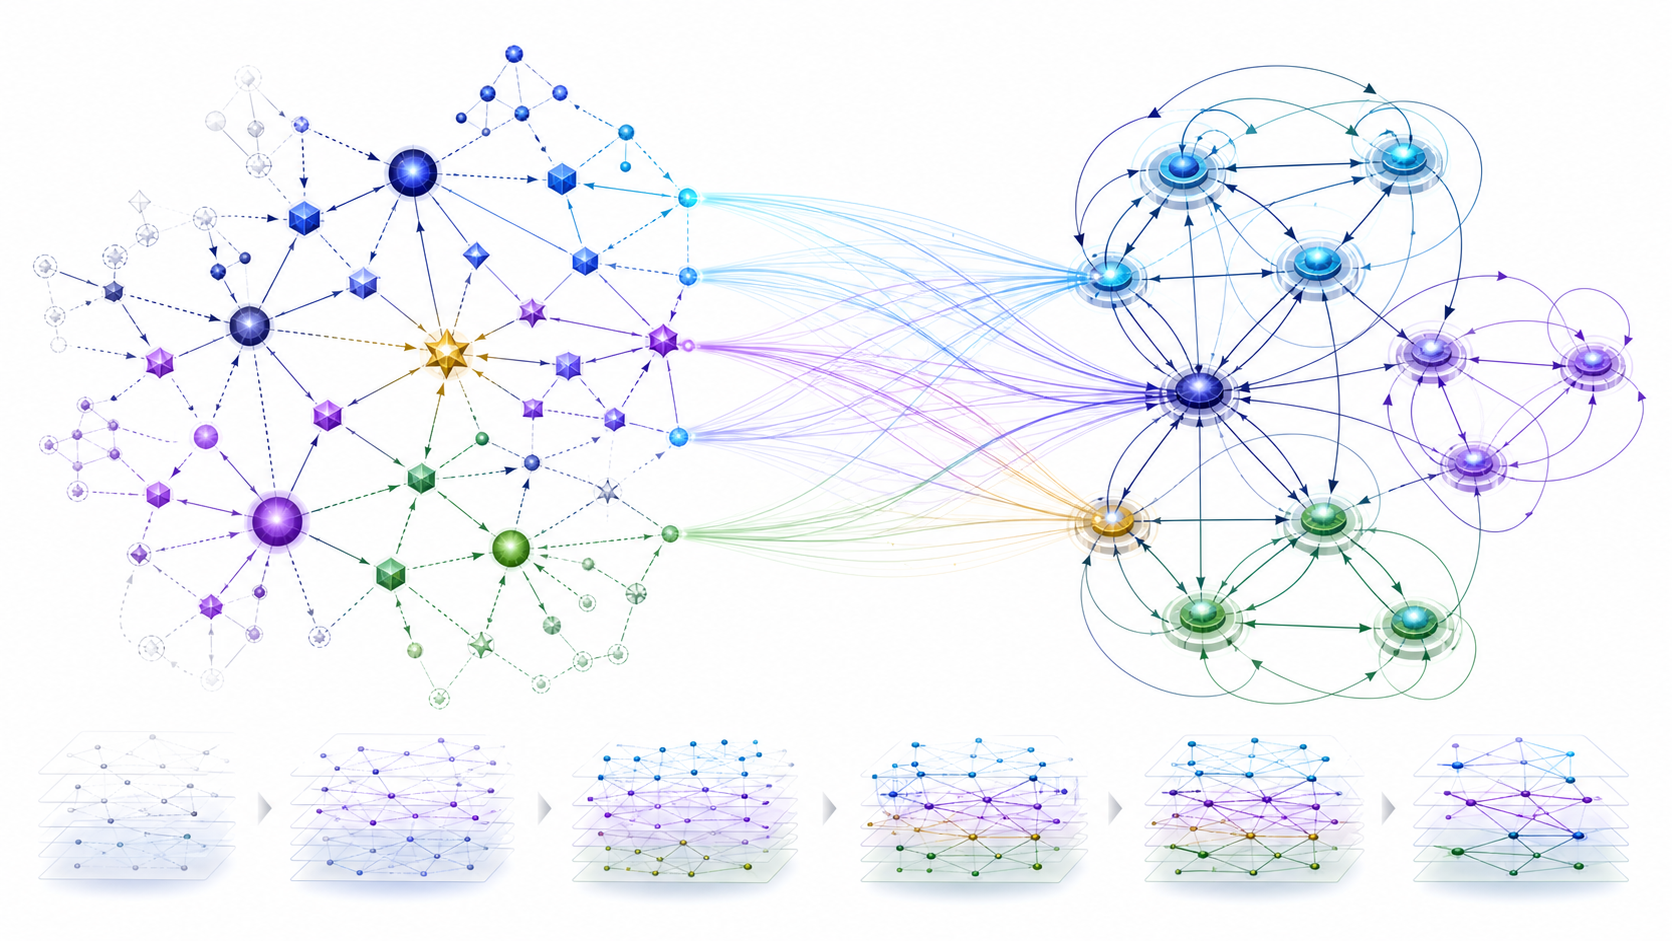
\includegraphics[width=.9\textwidth,height=.38\textheight,keepaspectratio]{images/cognitive-structure-functional-topology.png}
\caption{CSO 本体与 Agent-CSO 承载的分离}
\end{figure}
\section{CSO 不等于智能体内部的 Representation}

在讨论智能系统时，一个极其常见而又容易被忽略的概念错误，是把“某个对象在智能体内部的表示”直接等同于“该对象本身”。在现代人工智能系统中，这种等同尤其容易发生，因为我们几乎总是通过某种具体数据结构来接触所谓“知识”：token 序列、embedding、hidden state、key--value memory、knowledge graph node、vector database entry、neural activation pattern，甚至某段自然语言描述。于是，一个未经严格区分的理论很容易默认：
\[
\text{CognitiveObject}
=
\text{InternalRepresentation}.
\]
本书认为，这种等式在研究短时任务时尚可作为工程近似，但在研究持续智能、多主体比较和结构迁移时必须被取消。

我们首先把 CSO 定义为认知结构层上的对象。它可以是一个实体，也可以是一种关系、一条约束、一个事件、一个目标、一种因果结构、一个预测、一个计划、一项技能结构，乃至“我是谁”这一类自指结构。其关键并不在于采用何种数字编码，而在于它在认知关系网中具有何种结构角色。假定存在一个认知结构全集
\[
\mathcal C
=
\{C_1,C_2,\ldots,C_n,\ldots\},
\]
其中任意
\[
C_i\in\mathcal C
\]
均表示一个 CSO。我们允许 CSO 之间存在多种类型的关系：
\[
r_{ij}^{(k)}
:
C_i
\rightarrow
C_j,
\]
这里的上标 $k$ 可以分别表示语义关系、因果关系、时间关系、空间关系、约束关系、目标依赖关系、自我归属关系等。因此，从一开始我们面对的就不是一个无结构的“信息集合”，而是一张具有异质关系的认知结构图：
\[
\mathcal G_C
=
(\mathcal C,\mathcal R_C).
\]

这里必须特别强调，$\mathcal G_C$ 还不是某一个具体 Agent 大脑或软件运行时里的图。它是我们用来讨论“认知结构是什么”的理论层对象。就像“圆”不等于屏幕上绘制圆的像素集合，“某个目标与某项约束之间存在冲突”也不等于某一次 Transformer forward pass 中特定神经元的数值模式。后者可以承载前者，但二者并不因此获得同一性。

我们可以把这种区分写成：
\[
\boxed{
CSO\ Ontology
\neq
CSO\ Representation
}
\]
更准确地说，representation 是关于 CSO 的某种具体 realization。若某个智能体 $A$ 采用表示系统 $\mathcal R_A$，则存在映射
\[
\pi_A:
\mathcal C
\rightarrow
\mathcal R_A.
\]
于是同一个 CSO $C$ 可以在 $A$ 中表现为：
\[
\pi_A(C)=r_A.
\]
另一智能体 $B$ 可能采用完全不同的表示系统：
\[
\pi_B(C)=r_B.
\]
一般情况下，
\[
r_A\neq r_B,
\]
但这一事实本身并不要求
\[
C_A\neq C_B.
\]
如果二者保留了该 CSO 在相关认知任务中的关键结构关系，我们仍然可能认为它们是在承载“同一个认知结构”。

这一点对智能动力学极其重要。因为如果 representation 与 ontology 不分，我们以后所谓“学习”只能写成：
\[
r_t\rightarrow r_{t+1},
\]
却无法判断这种变化究竟意味着同一认知结构换了一种编码，还是认知结构本身发生了改变。例如，一位人类从用语言描述骑自行车，到形成高度自动化的程序性技能，其内部神经表示显然发生了巨大变化，但我们并不会因此认为“平衡自行车这一能力结构”已经变成完全无关的另一种东西。类似地，一个 Agent 最初通过显式自然语言计划完成网页操作，后来把重复步骤编译为 Skill 或 Program，也不能简单理解成原知识消失。更合理的描述是：
\[
\boxed{
Same\ CSO,\ Different\ Realization.
}
\]

从这里开始，我们能够第一次严格区分三种变化。第一种是表示变化：
\[
\Delta R\neq0,
\qquad
\Delta C\approx0.
\]
第二种是认知结构自身发生变化：
\[
\Delta C\neq0.
\]
第三种则是两者共同改变：
\[
\Delta C\neq0,
\qquad
\Delta R\neq0.
\]
后面的持续学习、记忆重构、技能形成和拓扑学习理论，都必须依赖这一基本区分。如果没有本体与表示的分离，我们看到的永远只是存储格式变化，而无法建立一门真正讨论认知结构演化的动力学理论。

从外部理论看，这一观点与哲学中的多重实现性、认知科学中的表征层级、计算机科学中的抽象数据类型和语义--实现分离存在亲缘关系；但本书并不直接等同于其中任何一种理论。我们的特殊目标是把这种区分引入持续智能的动力学描述，使后续能够进一步讨论：
\[
Representation,
\quad
Function,
\quad
Timescale,
\quad
Carrier,
\quad
Topology
\]
之间的联合迁移。也正因为如此，本章不会把 CSO 简化成 knowledge graph node，也不会把 Agent-CSO 简化成 embedding。它们分别属于不同理论层。

\section{Agent-CSO：CSO 在具体智能体中的实现}

如果说 CSO 回答的是“认知结构是什么”，那么 Agent-CSO 回答的就是“这个认知结构在某一个具体智能体中如何存在”。因此，我们正式定义一个智能体 $A$ 的实现映射：
\[
\pi_A:
\mathcal C
\rightarrow
\mathcal A_C,
\]
其中 $\mathcal A_C$ 表示该智能体能够承载的 Agent-CSO 状态空间。对于任意
\[
C\in\mathcal C,
\]
其在智能体 $A$ 中的具体实现记为：
\[
\boxed{
C_A
=
AgentCSO_A(C)
=
\pi_A(C).
}
\]

这个定义的核心不在符号，而在于它改变了我们观察智能内部世界的方式。传统知识表示通常把“一个知识单元”理解成某段可以读取或写入的数据；Agent-CSO 则要求我们把一个认知结构视为一个具有运行条件和动力属性的实体。同一个“门现在关闭”这样的结构，可能在视觉感知回路中以短寿命的空间状态存在，在工作记忆 $h(t)$ 中成为当前计划的显式约束，在情景记忆 $E$ 中成为某段行动轨迹的一部分，在结构记忆 $\Theta$ 中又可能沉降为“这种门需要先转动把手再推开”的一般技能结构。也就是说：
\[
C
\]
本体上可以保持一定连续性，而：
\[
AgentCSO_A(C)
\]
却会随着时间和功能位置发生迁移。

因此，我们不能把 Agent-CSO 定义成某个静态数组，而应写成时间相关对象：
\[
C_A(t)
=
AgentCSO_A(C,t).
\]
它至少要回答六个问题：它承载的是哪个 CSO；当前采用什么表示；当前由哪个功能区域处理；处于什么有效时间尺度；位于系统内部还是外部；当前处于激活、潜伏、预测、回忆还是其他运行状态。

由此，本书采用如下标准形式：
\[
\boxed{
AgentCSO_A(C,t)
=
\left(
C,
R_A,
F_A,
\tau_A,
B_A,
S_A
\right)_t
}
\]
其中：
\[
C
\]
表示本体 CSO；
\[
R_A
\]
表示智能体 $A$ 当前采用的具体 representation；
\[
F_A
\]
表示当前承担该 CSO 的功能位置；
\[
\tau_A
\]
表示这一实现当前有效的动力学时间尺度；
\[
B_A
\]
表示其承载边界或载体；
\[
S_A
\]
表示其运行状态。

这意味着，一个 Agent-CSO 从理论上首先是一个带坐标的动态实现，而不是孤立的“知识块”。其变化可以表示成：
\[
AgentCSO_A(C,t)
\rightarrow
AgentCSO_A(C,t+\Delta t).
\]
即使：
\[
C(t+\Delta t)\approx C(t),
\]
我们仍然可能有：
\[
R_A(t+\Delta t)\neq R_A(t),
\]
\[
F_A(t+\Delta t)\neq F_A(t),
\]
\[
\tau_A(t+\Delta t)\neq\tau_A(t),
\]
甚至：
\[
B_A(t+\Delta t)\neq B_A(t).
\]

例如，一个 Agent 第一次执行复杂软件流程时，某个操作结构可能以自然语言计划存在于工作记忆中：
\[
C_A^{(1)}
=
(C,R_{\text{text}},h,\tau_h,\text{internal},\text{active}).
\]
经过大量重复以后，它可能迁移成一个程序化 Skill：
\[
C_A^{(2)}
=
(C,R_{\text{policy}},F_{\text{skill}},\tau_{\text{fast}},
\text{external/service},\text{compiled}).
\]
从表面看，两者的数据格式、运行速度和承载位置都发生了改变；如果缺少 CSO/Agent-CSO 区分，我们很容易误认为这是两个互不相关的能力。采用本章框架后，我们反而可以明确指出：这是一条 Agent-CSO 生命周期轨迹。

这种写法还允许我们区分“当前未激活”与“不存在”。假定：
\[
S_A(C,t)=\text{latent},
\]
并不意味着：
\[
C\notin A.
\]
它可能只是暂时没有进入工作记忆。当检索、环境刺激或目标条件触发后：
\[
S_A:
\text{latent}
\rightarrow
\text{active}.
\]
这一点对于后续三相记忆理论尤其重要。$h$ 中的内容只是少量当前活跃 Agent-CSO，而不是智能体拥有的全部认知结构。

因此，本章提出一个重要原则：
\[
\boxed{
Agent\ Knowledge
\neq
Currently\ Active\ AgentCSO.
}
\]
成熟智能的大部分能力本来就应该处于非显式激活状态。只有真正需要跨功能全局协调的结构才需要进入 $h(t)$。这一原则将在后续工作记忆有限容量理论中进一步转化为工程约束。

\section{同一 CSO 的多种实现：Same CSO, Different Carrier}

当我们正式区分 CSO 与 Agent-CSO 以后，一个直接结果就是：认知结构不再被绑定于唯一材料、唯一算法甚至唯一功能模块。我们现在可以严谨表达：
\[
\boxed{
Same\ CSO
\neq
Same\ Carrier
}
\]
更进一步：
\[
\boxed{
Same\ CSO
\neq
Same\ Representation
\neq
Same\ Dynamics.
}
\]
这构成智能实现独立性理论最基本的一层。

考虑两个智能体 $A$ 和 $B$。对于同一个 CSO $C$，分别有：
\[
C_A=\pi_A(C),
\qquad
C_B=\pi_B(C).
\]
一般情况下，
\[
\pi_A(C)\neq\pi_B(C).
\]
这不仅意味着底层参数不同，还可能意味着表示范式完全不同。例如，$A$ 可能使用神经分布式表示，$B$ 可能使用符号图结构；$A$ 可能把某项能力固化在模型参数中，$B$ 可能通过外部 Skill 实现；$A$ 的有效闭环周期可能以秒为尺度，而 $B$ 的实现则可能以毫秒执行。只要我们仍能够建立适当的结构对应关系，就不能因为载体不同而直接断言两者面对的是不同 CSO。

我们可以引入一个结构保持映射：
\[
\Phi_{AB}:
AgentCSO_A(C)
\rightarrow
AgentCSO_B(C).
\]
它不要求：
\[
R_A=R_B,
\]
而要求对与任务相关的关键关系集合 $\mathcal R^\ast$ 满足近似保持条件：
\[
\Phi_{AB}
\left(
r_A(C_i,C_j)
\right)
\simeq
r_B
\left(
\Phi_{AB}(C_i),
\Phi_{AB}(C_j)
\right).
\]
因此真正重要的不是比特级相等，而是结构、功能和动力关系在合理容差内保持。

这使我们能够把“同一认知结构”理解成一种等价类。定义：
\[
AgentCSO_A(C)
\sim
AgentCSO_B(C)
\]
当且仅当二者在指定任务域 $\mathcal D$ 中保持足够的语义关系、功能闭环和行为约束。于是：
\[
[C]
=
\left\{
AgentCSO_X
\mid
AgentCSO_X\sim C
\right\}
\]
可以被理解成一个实现等价类。

这里我们必须避免走向另一个极端：只要最后行为类似，就宣称内部结构完全相同。两个系统都可以输出同样答案，却通过完全不同的因果结构产生结果。因此，我们需要区分至少三个层次的等价。

第一层是行为等价：
\[
\mathcal E_{beh}.
\]
它只要求在给定测试集上：
\[
Output_A\approx Output_B.
\]

第二层是功能等价：
\[
\mathcal E_{fun}.
\]
它要求系统中存在相似的预测、约束、记忆或控制作用。

第三层是结构动力等价：
\[
\mathcal E_{dyn}.
\]
它进一步要求关键 CSO 关系、跨时间尺度迁移方式和闭环结构可以建立映射。

通常有：
\[
\mathcal E_{dyn}
\Rightarrow
\mathcal E_{fun}
\Rightarrow
\mathcal E_{beh},
\]
反之并不必然成立。

这一层区分对于未来研究“人脑与人工智能是否属于同类智能”尤其重要。如果我们简单比较神经元与 Transformer，二者显然不同；如果只比较最终答案，又过于宽松。本书真正希望寻找的是：
\[
\boxed{
Multiscale\ Cognitive\ Dynamical\ Isomorphism
}
\]
即不同材料和实现是否能够在认知结构、功能闭环和时间尺度关系上形成近似同构。

这一观点也意味着，所谓 AgentOS 不应该把内部 representation ABI 固定成某一种模型特征空间。相反，系统标准应尽可能作用于更加稳定的语义和功能边界。例如后续 SGC、FCS、Body ABI、Control Reference 等设计，其重要性恰恰在于：它们提供的是相对稳定的功能语义接口，而不是要求所有内部模型共享同样 latent。

换言之，我们真正追求的是：
\[
\boxed{
Semantic/Functional\ Continuity
>
Representational\ Identity.
}
\]
这是后续 KRA 理论中“Functional Alignment $>$ Representation Alignment”的认识论前提，而其根源正是在本章完成的 CSO 与 Agent-CSO 分离。

\section{Agent-CSO 的五个实现坐标：表示、功能、时间尺度、边界与状态}

为了使 Agent-CSO 能够进入动力学分析，我们必须进一步展开：
\[
AgentCSO_A(C,t)
=
(C,R,F,\tau,B,S)_t.
\]
其中 $C$ 是理论本体锚点，而其余五个变量共同描述这一认知结构在当前 Agent 中“怎样存在”。本节依次讨论这五个实现坐标，并说明为什么后续所谓学习，本质上正是这些坐标的重新配置。

首先是表示坐标：
\[
R.
\]
它描述 CSO 以何种内部形式被编码。例如同一个空间约束可以通过自然语言、几何图、latent vector、symbolic rule、程序条件或训练参数实现。于是表示变化可以写成：
\[
M_R:
R_i
\rightarrow
R_j.
\]
这种变化并不必然改变 CSO 本体，而可能只是把同一结构从一种编码迁移到另一种更适合当前运行条件的编码。后续所谓抽象、压缩、程序化、参数化，很多都首先表现为 $M_R$。

第二是功能坐标：
\[
F.
\]
它回答“当前由哪个功能承担这一结构”。若系统功能集合为：
\[
V_F
=
\{F_1,F_2,\ldots,F_n\},
\]
则一个 Agent-CSO 在不同时刻可能具有：
\[
F(C,t)=F_i,
\]
以及：
\[
F(C,t+\Delta t)=F_j.
\]
这就是功能迁移：
\[
M_F:
F_i
\rightarrow
F_j.
\]
例如初学技能需要高层显式规划，熟练以后转移到低层技能控制器。后面的“复杂度向下沉降”在本体修正后，其实主要就是 Agent-CSO 的功能位置迁移。

第三是时间尺度坐标：
\[
\tau.
\]
一个认知结构并不只有“存在或不存在”，它还以某种特征时间尺度发挥作用。当前工作记忆中的 Agent-CSO 可能具有：
\[
\tau\sim \tau_h,
\]
情景经验可能具有：
\[
\tau\sim\tau_E,
\]
结构记忆则可能具有：
\[
\tau\sim\tau_\Theta.
\]
如果某个结构从快速显式活动沉降为慢速稳定生成结构，则：
\[
M_\tau:
\tau_{\text{fast}}
\rightarrow
\tau_{\text{slow}}.
\]
反过来，召回过程则可以理解为：
\[
\tau_{\text{slow}}
\rightarrow
\tau_{\text{fast}}.
\]
由此可见，记忆并不只是“存入某个数据库”，而是认知结构在时间尺度空间中的重新分布。

第四是边界或承载坐标：
\[
B.
\]
这里我们允许：
\[
B
\in
\{
Internal,
Skill,
Tool,
File,
Database,
Program,
Environment,
OtherAgent,
\ldots
\}.
\]
当一个 Agent 不再在内部显式维持完整结构，而是把它转移到程序、工具、外部文件或环境结构时，我们写：
\[
M_B:
B_{\text{internal}}
\rightarrow
B_{\text{external}}.
\]
这为后续认知卸载理论建立了更严谨的本体基础。所谓 Offloading，不再是神秘的“把复杂度扔出去”，而是：
\[
\boxed{
AgentCSO\ Carrier\ Migration.
}
\]

第五是状态坐标：
\[
S.
\]
典型取值可以包括：
\[
S
\in
\{
active,
latent,
retrieved,
predicted,
counterfactual,
compiled,
suppressed,
uncertain,
\ldots
\}.
\]
这一维尤其重要，因为它区分“当前活跃”与“长期存在”。例如一个 Agent 可能拥有某项结构知识，但在当前任务中完全未激活：
\[
S=\text{latent}.
\]
当情景匹配后：
\[
\text{latent}
\rightarrow
\text{retrieved}
\rightarrow
\text{active}.
\]
完成后又可能：
\[
\text{active}
\rightarrow
\text{consolidated}.
\]

因此，我们能够定义 Agent-CSO 的完整迁移向量：
\[
\boxed{
\mathcal M_{CSO}
=
\left(
M_R,
M_F,
M_\tau,
M_B,
M_S
\right).
}
\]
这比早期单纯“复杂度迁移”的表述更加精确。复杂度可以作为这些迁移过程中的负载测量量，但真正发生变化的是认知结构的 realization coordinates。

这一形式还提供了一种以后进行实证测量的可能。若能够追踪某个 CSO 在 Agent 生命周期中的：
\[
\Gamma_C(t)
=
\big(
R(t),F(t),\tau(t),B(t),S(t)
\big),
\]
则：
\[
\Gamma_C
\]
就是它的 Agent-CSO 生命周期轨迹。我们甚至可以比较不同 Agent 的同一 CSO 轨迹：
\[
\Gamma_C^A(t),
\qquad
\Gamma_C^B(t),
\]
研究为什么某种架构更容易形成自动化技能，为什么另一种架构长期停留在高成本显式认知层。这使“学习效率”从最终准确率进一步拓展为“结构如何改变承载方式”的动力学问题。

\section{Agent-CSO 的标准状态描述与动力学形式化}

在建立五个实现坐标以后，我们可以正式给 Agent-CSO 提供一个更完整的数学对象。设智能体 $A$ 的状态空间为：
\[
\mathcal X_A
=
\mathcal X_R
\times
\mathcal X_F
\times
\mathcal X_\tau
\times
\mathcal X_B
\times
\mathcal X_S.
\]
对于 CSO $C$，定义其 Agent 内部 realization state：
\[
x_C^A(t)
=
\left[
r_C(t),
f_C(t),
\tau_C(t),
b_C(t),
s_C(t)
\right]^\top.
\]
于是：
\[
AgentCSO_A(C,t)
=
(C,x_C^A(t)).
\]

在最一般情况下，其动力学可表示为：
\[
\dot x_C^A
=
F_C
\left(
x_C^A,
\mathcal N_C,
h,
E,
\Theta,
\Psi,
G,
W,
u,
\xi
\right),
\]
其中：
\[
\mathcal N_C
\]
表示与 $C$ 相邻的其他 Agent-CSO；
$h,E,\Theta,\Psi$ 分别表示后续章节将展开的工作记忆、情景记忆、结构记忆和慢速自我约束；
$G$ 表示当前目标；
$W$ 表示外部世界状态；
$u$ 表示认知或行动控制输入；
$\xi$ 表示随机扰动和不可观测影响。

这一写法具有一个重要意义：一个 Agent-CSO 从来不是孤立更新的。认知结构变化通常来自关系网络，因此更一般地，我们应考虑：
\[
\mathcal G_C^A(t)
=
\left(
V_C^A(t),
E_C^A(t)
\right),
\]
其中每个节点：
\[
v_i
=
AgentCSO_A(C_i,t).
\]
于是其动力学是耦合系统：
\[
\dot x_i
=
F_i
\left(
x_i,
\{x_j:j\in\mathcal N_i\},
u_i,
w_i
\right).
\]

这使我们能够第一次把“知识改变”与“认知结构动力学”区分开。知识数据库中的修改通常表现为：
\[
value_i
\leftarrow
value_i',
\]
而真正持续 Agent 的认知变化可能同时涉及：
\[
R_i,\quad
F_i,\quad
\tau_i,\quad
B_i,\quad
S_i
\]
的耦合变化。一个结构被认为“学会了”，并不一定因为它的数据表示变得更精确；也可能因为它已经从高延迟显式推理迁移到了快速稳定闭环。

我们可以进一步定义一个 Agent-CSO 的功能成本：
\[
J_C
=
\int_{t_0}^{t_1}
\left[
\lambda_h L_h(C,t)
+
\lambda_e E_C(t)
+
\lambda_r R_C(t)
+
\lambda_\ell Latency_C(t)
\right]dt,
\]
其中：
\[
L_h
\]
表示该结构占用全局工作记忆的负载，
\[
E_C
\]
表示计算或能量成本，
\[
R_C
\]
表示误差/风险，
\[
Latency_C
\]
表示响应时延。

这样我们就能形式化一个极其重要的学习直觉：如果某个 CSO 长期重复出现，系统会倾向寻找能够降低长期成本的 realization：
\[
x_C^\ast
=
\arg\min_{x_C}
\mathbb E[J_C].
\]
这可能意味着：
\[
F_{\text{explicit}}
\rightarrow
F_{\text{procedural}},
\]
或者：
\[
B_{\text{internal}}
\rightarrow
B_{\text{tool}},
\]
甚至：
\[
R_{\text{verbose}}
\rightarrow
R_{\text{compressed}}.
\]

这正是后续 Skill Formation、Offloading 和 Topological Learning 能够统一在同一理论框架中的原因。

我们还需要定义 CSO 与 realization 的连续性判据。由于实际学习会发生抽象和重构，所以不能要求：
\[
R_t=R_{t+\Delta}.
\]
更合理的是给出结构保持函数：
\[
\kappa_C
\left(
AgentCSO_t,
AgentCSO_{t+\Delta}
\right)
\in[0,1].
\]
当：
\[
\kappa_C>\theta_C,
\]
我们认为两者仍然属于同一 CSO 的连续 realization；当：
\[
\kappa_C\leq\theta_C,
\]
则可能已经发生结构分裂、合并或本体改变。

这里的 $\kappa_C$ 不应被理解成一个固定 cosine similarity，而应综合：
\[
\resizebox{.96\linewidth}{!}{$\displaystyle
SemanticConsistency,
\quad
FunctionalConsistency,
\quad
RelationalConsistency,
\quad
CausalConsistency.
$}
\]
这一点会在未来真正实现 Agent-CSO tracking 时非常关键，因为“表示相似”远弱于“结构连续”。

因此，本书今后讨论任何认知结构变化时，都可以遵循一个统一描述：
\[
\boxed{
C
\quad+\quad
x_C^A(t)
\quad+\quad
\dot x_C^A(t)
}
\]
即同时说明：我们讨论的结构是什么；它当前如何被承载；它正在怎样变化。

\section{同一现实为何会形成不同智能体的内部世界}

CSO 与 Agent-CSO 的分离自然引出一个认识论问题：如果多个智能体面对同一个现实，它们为什么仍然可以拥有完全不同的内部世界？答案并不只是“它们的模型参数不同”，而是因为从 CSO 到 Agent-CSO 的映射本身就是依赖主体结构的投影过程。

设存在某一认知结构：
\[
C\in\mathcal C.
\]
智能体 $A$ 与 $B$ 分别具有：
\[
\pi_A:C\rightarrow AgentCSO_A(C),
\]
以及：
\[
\pi_B:C\rightarrow AgentCSO_B(C).
\]
通常：
\[
\pi_A\neq\pi_B.
\]
原因至少来自五个方面。

第一，观察界面不同。不同身体、感知器官和传感器决定哪些结构能够进入内部世界。若：
\[
O_A(W)\neq O_B(W),
\]
即使二者处于同一个外部环境，得到的初始证据也不同。

第二，历史不同。智能体已有的：
\[
E_A,\Theta_A
\]
与：
\[
E_B,\Theta_B
\]
不同，因此新证据会被不同结构解释。一个新事件 $e$ 的内部结构并不是简单：
\[
AgentCSO=e,
\]
而更接近：
\[
AgentCSO_A(e)
=
\Phi(e,E_A,\Theta_A,\Psi_A).
\]

第三，自我与价值结构不同。后续我们将定义：
\[
\Psi_A
\]
作为智能体的慢速身份与价值约束，因此同一事件对不同 Agent 的意义不同。也就是说，Agent-CSO 不只是“外界结构的副本”，而是外界证据与既有主体结构共同生成的结果。

第四，功能拓扑不同。若某个 Agent 具有专门处理空间关系的稳定闭环，而另一个 Agent 需要经过显式语言推理，那么同一个 CSO 的：
\[
F_A(C)\neq F_B(C),
\]
以及：
\[
\tau_A(C)\neq\tau_B(C).
\]
这意味着内部世界不仅“内容不同”，连处理该内容的动力学结构也不同。

第五，行动能力不同。一个结构是否重要，往往取决于它与行动的关系。例如同一个楼梯对于人形机器人和轮式机器人虽然可以共享部分几何 CSO，但其 affordance 结构显然不同：
\[
C_{\text{stairs}}^{human}
\neq
C_{\text{stairs}}^{wheel}
\]
至少在可行动关系层上如此。因此，一个智能体内部世界从一开始就是：
\begin{statementbox}
RealityRelativeToThisAgent.
\end{statementbox}

这说明：
\[
AgentWorld_A
\neq
AgentWorld_B
\]
并不必然意味着其中一个“错误”。真正需要进一步判断的是：
\[
\mathcal F_A
=
\text{Functional adequacy of }AgentWorld_A,
\]
即这个内部世界能否支持有效预测、决策和行动。

从概率角度可以写：
\[
p_A(C\mid o_{1:t},E_A,\Theta_A,\Psi_A)
\]
与：
\[
p_B(C\mid o_{1:t},E_B,\Theta_B,\Psi_B).
\]
即使：
\[
o_{1:t}^{A}=o_{1:t}^{B},
\]
后验也未必相同。

这一点对以后“真理”“世界模型”和“自我模型”讨论具有重要意义。我们的理论不会要求 Agent 内部存在一个与现实逐点同构的微型宇宙。事实上，由于工作记忆有限、感知有限和计算有限，完整复制现实本身既不可能，也没有必要。智能所需要的是：
\[
\boxed{
Action\text{-}Sufficient\ Structural\ Representation.
}
\]
即在当前身体、目标和时间尺度下足以支撑正确闭环的结构表示。

因此，本章的认识论立场不是朴素镜像论：
\[
InternalWorld
=
Copy(ExternalWorld),
\]
而更接近：
\[
\boxed{
InternalWorld
=
AgentConditionedStructuralProjection(Reality).
}
\]
这种投影必须受到现实不断校正，但不要求与现实具有相同物理形式。

这也解释了为什么后续 SGC 会被定义成 Body-Centered Semantic Reality，而不是客观宇宙数据库；为什么 FCS 描述的是“现实如何影响我”，而不是现实自身的全部性质；以及为什么 $\Psi$ 会参与记忆筛选。智能体内部世界从来不是无主体的世界复制，而是现实结构进入一个有限、具身、具有历史与目标的持续主体后形成的 Agent-CSO 网络。

\section{Representation Independence：实现独立性及其边界}

CSO 与 Agent-CSO 的区分最终使我们能够提出实现独立性原则：
\[
\boxed{
CognitiveOntology
\ \text{is not uniquely determined by}\
ImplementationSubstrate.
}
\]
这意味着，一个认知结构是否存在，原则上不能只依据它由神经元、Transformer、symbolic graph、程序还是其他未知物理载体实现来判断。实现材料当然会约束动力学，但它不是认知结构分类的唯一标准。

形式上，设：
\[
A=(\mathcal G_C^A,\mathcal G_F^A,\mu_A),
\]
\[
B=(\mathcal G_C^B,\mathcal G_F^B,\mu_B),
\]
分别表示两个智能体的认知图、功能图及其动态承载映射。若存在：
\[
\Phi_C:
\mathcal G_C^A
\rightarrow
\mathcal G_C^B,
\]
以及：
\[
\Phi_F:
\mathcal G_F^A
\rightarrow
\mathcal G_F^B,
\]
使主要关系满足：
\[
\Phi_C(r_{ij}^A)
\simeq
r_{ij}^B,
\]
主要功能闭环满足：
\[
\Phi_F(L_k^A)
\simeq
L_k^B,
\]
并且二者时间尺度存在单调映射：
\[
\tau_B
=
g(\tau_A),
\qquad
g'(\tau)>0,
\]
那么即便底层实现完全不同，我们仍可以说两个系统在指定研究尺度上具有：
\[
\boxed{
Multiscale\ Cognitive\ Dynamical\ Isomorphism.
}
\]

这一概念比传统“功能主义”要求更强，因为我们并不只要求输入输出相同，还希望保留多尺度状态迁移和功能闭环关系。例如，两个系统都能识别危险并避开它，并不足以说明它们具有完全相同的认知结构。如果一个系统只是硬编码条件反射，另一个系统则具有情景记忆、自我状态估计、预测与长期价值调节，那么它们的宏观行为在部分场景中可能相同，但内部动力学并不同构。

因此，实现独立性绝不是：
\[
Anything\ That\ Behaves\ Similarly
=
Same\ Intelligence.
\]
更合理的是分层判断。

定义行为保持度：
\[
D_B(A,B),
\]
语义结构保持度：
\[
D_C(A,B),
\]
功能闭环保持度：
\[
D_F(A,B),
\]
多尺度迁移保持度：
\[
D_M(A,B).
\]
则可以构造一个概念性的智能同构指标：
\[
\mathcal I_{AB}
=
w_BD_B
+
w_CD_C
+
w_FD_F
+
w_MD_M,
\]
其中：
\[
\sum_i w_i=1.
\]
不同研究问题可以赋予不同权重。研究工具执行系统时，行为和功能权重可能较高；研究长期身份连续时，CSO 结构和慢尺度迁移可能更重要。

这里还有一个重要边界：实现独立不意味着实现无关。不同材料仍会影响：
\[
Latency,
\quad
Noise,
\quad
Energy,
\quad
Plasticity,
\quad
Reliability,
\quad
Scalability.
\]
所以更准确的命题是：
\[
\boxed{
Ontology\ is\ not\ reducible\ to\ substrate,
\quad
Dynamics\ remain\ substrate\ constrained.
}
\]
即认知本体不被某一种材料唯一决定，但其实际动力学始终受实现材料约束。

这一原则对于 AgentOS 工程具有直接后果。我们应尽量让 Agent Kernel 的高级语义依赖：
\[
CSO/Function/Timescale
\]
而不是特定模型 latent；让 Body Runtime 的接口依赖：
\[
SGC,\ FCS,\ ControlReference
\]
而不是特定机器人厂商的内部表示；让 KRA 负责在不同 representation 之间维护功能关系。这样，系统才有可能跨模型、跨身体、跨硬件发展。

换句话说，真正能够跨世代持续发展的智能架构，其稳定对象不应该是每一代神经网络的参数格式，而应该是更高层的：
\[
\boxed{
Cognitive\ Contracts.
}
\]
这些 contract 描述“什么结构必须被表达”“什么闭环必须成立”“什么现实反馈必须返回”，而允许内部实现不断变化。

\section{CSO--Agent-CSO 区分与同类智能判定}

本章最终要回到一个更大的认识论问题：为什么区分 CSO 与 Agent-CSO，能够帮助我们判断两个完全不同的系统是否属于“同类智能”？答案是，如果没有这种区分，我们只能在两个极端中选择：要么比较底层材料，要么比较外部行为。前者过于严格，后者又过于宽松。CSO/Agent-CSO 提供了一层介于两者之间、同时具有结构与动力意义的比较坐标。

设两个智能体：
\[
A,\qquad B.
\]
我们首先不要求：
\[
Parameters_A
=
Parameters_B,
\]
也不要求：
\[
Architecture_A
=
Architecture_B.
\]
相反，我们考察是否存在一组关键 CSO：
\[
\mathcal C^\ast
=
\{C_1,\ldots,C_m\},
\]
使二者都能够形成对应的 Agent-CSO：
\[
\pi_A(C_i),
\qquad
\pi_B(C_i).
\]
然后进一步考察这些 Agent-CSO 之间的关系是否保持。

例如，如果任务要求识别：
\[
Object,
\quad
Threat,
\quad
Goal,
\quad
Self,
\quad
Constraint,
\]
那么我们不仅比较是否输出正确动作，还比较：
\[
Threat
\rightarrow
GoalModification,
\]
\[
Constraint
\rightarrow
PlanRestriction,
\]
\[
SelfState
\rightarrow
RiskAdjustment
\]
等结构关系是否存在。

因此，同类智能判定可以写成一个四层结构：

第一层，\textbf{问题空间同类性}：
\[
\mathcal D_A
\simeq
\mathcal D_B.
\]

第二层，\textbf{主要 CSO 类型同类性}：
\[
\mathcal C_A^\ast
\simeq
\mathcal C_B^\ast.
\]

第三层，\textbf{主要关系与功能闭环同类性}：
\[
\mathcal R_A^\ast
\simeq
\mathcal R_B^\ast.
\]

第四层，\textbf{多尺度迁移规律同类性}：
\[
\mathcal M_A^\ast
\simeq
\mathcal M_B^\ast.
\]

于是：
\[
\boxed{
Same\ Intelligence\ Class
\Rightarrow
Semantic\text{-}Functional\text{-}Dynamical\ Correspondence
}
\]
而不是要求材料同一。

这一框架也使我们此前提出的“语义类规约”获得更严格解释。所谓优先覆盖更多语义类型，并不是简单增加分类标签，而是使系统能够形成更多具有稳定关系的 CSO 类，并能够把这些类绑定到适当功能和时间尺度。一个系统如果只在表面行为上覆盖大量任务，但每一次都依赖同一个巨大中央推理过程，那么它与一个已经形成大量局部闭环、稳定技能和长期结构的成熟系统，在认知动力学意义上仍然可能属于不同阶段。

由此，本书可以提出一个重要区别：
\[
\boxed{
Capability\ Breadth
\neq
Structural\ Generality.
}
\]
前者表示系统能够完成多少任务，后者则表示系统能否形成、迁移、稳定和重新组织足够丰富的 Agent-CSO。

这也是后面讨论 AGI“通用性”时必须保留的基础。真正的通用智能不能只定义为：
\[
N_{\text{tasks}}\rightarrow\text{large},
\]
而更应该观察：
\begin{statementbox}
AbilityToConstructAndReorganizeAgentCSO
\end{statementbox}
是否足够强。换句话说，通用性不是简单拥有一个巨大的已有能力集合，而是能够在新现实中形成新的结构，并找到适当的 representation、function、timescale 和 carrier。

至此，我们可以给本章一个最终总结。CSO 代表认知结构层的对象：
\[
C\in\mathcal C.
\]
Agent-CSO 代表某个具体 Agent 对这一结构的动态 realization：
\[
AgentCSO_A(C,t)
=
(C,R,F,\tau,B,S)_t.
\]
学习首先可以表现为：
\[
(R,F,\tau,B,S)_t
\rightarrow
(R,F,\tau,B,S)_{t+\Delta t},
\]
而不要求 CSO 本体同时改变。反之，当关系结构本身发生长期重构时：
\[
C
\rightarrow
C',
\]
我们才进入真正的认知结构变化。

因此，本章完成了从“表示论”向“结构动力学”的关键过渡：
\[
\boxed{
Representation
\rightarrow
AgentCSO
\rightarrow
CSODynamics.
}
\]

下一章我们将面对一个历史上首先以“复杂度迁移”形式出现的问题：当一个认知结构不断改变其表示、功能位置、时间尺度和承载边界时，我们应该如何描述这种变化？早期理论把它解释为“复杂度在系统内部迁移”；在完成本章的本体分离以后，我们将看到，更基本的对象其实是：
\begin{statementbox}
\centering\bfseries
CSO 的承载结构正在迁移。
\end{statementbox}
这将成为从复杂度迁移理论转向认知结构迁移理论的理论转折点。
